% !TeX program = xelatex

\documentclass[11pt,a4paper]{article}

% -------------------------------
% Paquetes
% -------------------------------
\usepackage{iftex}
\ifPDFTeX
  \usepackage[utf8]{inputenc}
  \usepackage[T1]{fontenc}
  \IfFileExists{lmodern.sty}{\usepackage{lmodern}}{}
\else
  \usepackage{fontspec}
  \setmainfont{Latin Modern Roman}
\fi

\usepackage[spanish,es-nodecimaldot]{babel}
\usepackage{amsmath,amssymb}
\usepackage{graphicx}
\usepackage{booktabs}
\usepackage{longtable}
\usepackage{array}
\usepackage{geometry}
\usepackage[hypertexnames=false]{hyperref}
\usepackage{float}
\usepackage{caption}
\usepackage{subcaption}
\usepackage{fancyhdr}
\usepackage{xcolor}

\graphicspath{{figures/}{../figures/}{report/figures/}}

\geometry{margin=2.5cm}

\setlength{\parindent}{0pt}
\setlength{\parskip}{6pt}
\setlength{\headheight}{42pt}
\setlength{\headsep}{18pt}

\hypersetup{
  colorlinks=true,
  linkcolor=black,
  urlcolor=blue,
  citecolor=black
}
\urlstyle{tt}
\renewcommand{\figureautorefname}{Figura}
\renewcommand{\tableautorefname}{Cuadro}

\newcommand{\pendiente}[1]{\textcolor{red}{[Pendiente: #1]}}
\newcommand{\reportheader}{%
\begin{minipage}{\textwidth}
\vspace{6pt}
\makebox[\textwidth][s]{Trabajo Práctico N.\textdegree~3\hfill Series de Tiempo}
\vspace{6pt}
\hrule height 0.4pt
\end{minipage}%
}

\fancypagestyle{tpstyle}{%
  \fancyhf{}
  \fancyhead[C]{\reportheader}
  \fancyfoot[C]{\thepage}
  \renewcommand{\headrulewidth}{0pt}
  \renewcommand{\footrulewidth}{0pt}
}

\fancypagestyle{plain}{%
  \fancyhf{}
  \fancyhead[C]{\reportheader}
  \fancyfoot[C]{\thepage}
  \renewcommand{\headrulewidth}{0pt}
  \renewcommand{\footrulewidth}{0pt}
}

\pagestyle{tpstyle}

% -------------------------------
% Título
% -------------------------------
\title{%
\textbf{Elasticidades del comercio exterior argentino: extensión multivariada con modelos VAR y VEC} \\
\vspace{0.6em}
\large Trabajo Práctico N.\textdegree~3 - Series de Tiempo
}

\author{
Maestría en Economía Aplicada \\
Facultad de Ciencias Económicas - UBA \\
\\
\textbf{Integrantes:} \\
Andrea Chasi \\
Julián Delgadillo Marín \\
Christian Arias \\
Leonardo Ávila \\
\\
\textbf{Docente:} \\
Julio Eduardo Fabris
}

\date{\textbf{Fecha de entrega:} 27 de junio de 2026}

\begin{document}

\maketitle

% -------------------------------
% Resumen
% -------------------------------
\begin{abstract}
Este trabajo estima elasticidades de corto y largo plazo del comercio exterior
argentino mediante una extensión multivariada de los resultados obtenidos en el
Trabajo Práctico N.\textdegree~2. La estrategia combina el enfoque
uniecuacional de Engle-Granger y modelos de corrección del error con pruebas de
cointegración de Johansen, modelos VEC y modelos VAR en diferencias. El objetivo
es distinguir qué resultados pueden interpretarse como elasticidades de
equilibrio de largo plazo y cuáles deben leerse como evidencia dinámica de corto
plazo o como resultados indicativos. La evidencia preliminar respalda una
relación de largo plazo para importaciones, mientras que para exportaciones la
evidencia de cointegración es más débil y exige una interpretación cautelosa.
\end{abstract}

\newpage

% -------------------------------
% 1. Introducción
% -------------------------------
\section{Introducción}
\label{sec:introduccion}

El objetivo del informe es estimar las elasticidades del comercio exterior
argentino y evaluar su consistencia bajo distintas metodologías de series de
tiempo. En particular, se analizan las respuestas de las importaciones reales
al producto interno y al tipo de cambio real, y las respuestas de las
exportaciones reales a la demanda externa y al tipo de cambio real. El interés
económico de estas elasticidades radica en su vínculo con la restricción
externa: si las importaciones reaccionan con mayor intensidad al crecimiento
doméstico que las exportaciones a la demanda externa, la expansión del nivel de
actividad puede tensionar la disponibilidad de divisas.

El Trabajo Práctico N.\textdegree~3 completa el análisis desarrollado en el
Trabajo Práctico N.\textdegree~2. Por esa razón, el informe no reemplaza la
etapa Engle-Granger/ECM, sino que la incorpora como punto de comparación y la
extiende mediante herramientas multivariadas VAR/VEC. La consigna requiere
evaluar la existencia de raíces unitarias, cointegración por Engle-Granger y
Johansen, elasticidades de largo plazo cuando haya evidencia de equilibrio y
elasticidades de corto plazo mediante modelos con variables diferenciadas. Aun
cuando la evidencia de cointegración no sea concluyente, los resultados deben
reportarse con fines indicativos y compararse con la literatura aplicada para
Argentina.

% -------------------------------
% 2. Marco teórico
% -------------------------------
\section{Marco teórico económico}
\label{sec:marco-teorico}

El punto de partida son las ecuaciones tradicionales de demanda de importaciones
y exportaciones. Para importaciones, la relación básica puede escribirse como:

\begin{equation}
  M_t = f(Y_t, TCR_t),
\end{equation}

donde $M_t$ representa las importaciones reales, $Y_t$ el producto interno y
$TCR_t$ el tipo de cambio real. En logaritmos, la especificación empírica queda:

\begin{equation}
  \log(M_t) = \alpha_0 + \alpha_1 \log(Y_t) +
  \alpha_2 \log(TCR_t) + u_t.
  \label{eq:importaciones-largo-plazo}
\end{equation}

Para exportaciones, la ecuación clásica vincula las ventas externas con la
demanda internacional y el tipo de cambio real:

\begin{equation}
  \log(X_t) = \beta_0 + \beta_1 \log(Y_t^*) +
  \beta_2 \log(TCR_t) + \varepsilon_t,
  \label{eq:exportaciones-largo-plazo}
\end{equation}

donde $X_t$ son las exportaciones reales e $Y_t^*$ representa el producto global
o de los principales socios comerciales.

En estas ecuaciones, $\alpha_1$ mide la elasticidad ingreso de las importaciones
y $\beta_1$ la elasticidad de las exportaciones respecto de la demanda externa.
Los coeficientes asociados al tipo de cambio real capturan la sensibilidad de
los flujos comerciales ante cambios en precios relativos. En principio, se
espera que las importaciones respondan positivamente al producto interno y que
las exportaciones respondan positivamente a la demanda externa. El signo del
tipo de cambio real depende de la definición utilizada para el índice y debe
interpretarse de forma consistente con esa convención.

Desde el punto de vista macroeconómico, estas elasticidades son relevantes
porque permiten evaluar la relación entre crecimiento económico y restricción
externa. Si las importaciones presentan una elasticidad ingreso elevada, una
expansión del producto interno tiende a aumentar de manera significativa la
demanda de divisas asociada a compras externas. En cambio, si las exportaciones
responden con menor intensidad al crecimiento de la demanda externa o al tipo de
cambio real, la economía puede enfrentar dificultades para generar las divisas
necesarias para sostener un proceso de crecimiento.

En este sentido, la comparación entre elasticidades de importaciones y
exportaciones permite analizar si existe una asimetría estructural en el comercio
exterior argentino. Una elasticidad ingreso de las importaciones superior a la
elasticidad de las exportaciones respecto de la demanda externa implica que, ante
un proceso de expansión, las compras externas pueden crecer más rápido que las
ventas externas. Este patrón es consistente con la literatura sobre restricción
externa y con la idea de que el crecimiento argentino puede verse limitado por
la disponibilidad de divisas.

El tipo de cambio real cumple un papel adicional como precio relativo entre
bienes domésticos y externos. Una depreciación real debería, en principio,
encarecer las importaciones y mejorar la competitividad de las exportaciones.
Sin embargo, la magnitud de estas respuestas depende de la estructura productiva,
del contenido importado de la actividad, de la composición sectorial de las
exportaciones y de las condiciones de demanda internacional. Por ello, el efecto
del tipo de cambio real puede ser menor o más inestable que el efecto del ingreso
o de la demanda externa.

% -------------------------------
% 3. Marco metodológico
% -------------------------------
\section{Marco metodológico}
\label{sec:marco-metodologico}

El trabajo estima elasticidades de largo y corto plazo del comercio exterior
argentino mediante una estrategia que combina modelos uniecuacionales y modelos
multivariados. El punto de partida es el análisis realizado en el Trabajo
Práctico N.\textdegree~2, basado en relaciones de cointegración de
Engle-Granger y modelos de corrección del error. La extensión central de este
informe consiste en evaluar las mismas relaciones dentro de sistemas VAR/VEC,
utilizando la metodología de Johansen para determinar el número de vectores de
cointegración.

La estrategia metodológica sigue la presentación de series integradas,
cointegración y modelos vectoriales desarrollada en Enders
\cite{enders_2014}, Hamilton \cite{hamilton_1994}, Lütkepohl
\cite{lutkepohl_2005}, Pfaff \cite{pfaff_2008}, Johansen
\cite{johansen_1995}, Engle y Granger \cite{engle_granger_1987}, Song, Witt y
Li \cite{song_witt_li_2008} y las notas de clase \cite{fabris_2026}. La lógica
general es no imponer una relación de equilibrio en niveles antes de verificar
el orden de integración de las series y la existencia de cointegración. Por
ello, el trabajo distingue explícitamente entre elasticidades de largo plazo,
asociadas a vectores de cointegración, y elasticidades de corto plazo, asociadas
a modelos en diferencias.

Todas las variables reales se transforman a logaritmos naturales. Para una
variable positiva \(Z_t\), la transformación se define como:

\begin{equation}
z_t = \ln(Z_t)
\label{eq:tp3-transformacion-logaritmica}
\end{equation}

Esta transformación permite interpretar los coeficientes de las relaciones en
niveles como elasticidades. Las variaciones trimestrales se aproximan mediante
primeras diferencias logarítmicas:

\begin{equation}
\Delta z_t = z_t - z_{t-1}
\label{eq:diferencia-logaritmica}
\end{equation}

En el caso de exportaciones, la demanda externa se aproxima mediante un índice
de producto de socios comerciales. Siguiendo el criterio utilizado en el TP 2,
el indicador se construye como una combinación ponderada en logaritmos de los
PIB de Brasil y Estados Unidos:

\begin{equation}
\ln(PIBSOCIOS_t)
= w_{BR}\ln(PIB_{BR,t}) + w_{US}\ln(PIB_{US,t})
\label{eq:tp3-pib-socios}
\end{equation}

La especificación de largo plazo para importaciones es la presentada en
\eqref{eq:importaciones-largo-plazo}. En esa ecuación, el coeficiente asociado
al producto interno mide la elasticidad ingreso de las importaciones, mientras
que el coeficiente del tipo de cambio real resume la elasticidad frente a
precios relativos. Para exportaciones se utiliza la relación de largo plazo
\eqref{eq:exportaciones-largo-plazo}, donde el producto de socios comerciales
aproxima la demanda externa relevante.

Antes de estimar relaciones en niveles se evalúa el orden de integración de las
series. La hipótesis central es que las variables macroeconómicas utilizadas en
las ecuaciones de comercio exterior pueden ser no estacionarias en niveles y
estacionarias en primeras diferencias. El análisis se inicia con pruebas
Dickey-Fuller aumentadas (ADF), aplicadas sobre niveles logarítmicos y primeras
diferencias logarítmicas. En niveles se consideran especificaciones con
tendencia determinística cuando corresponde, mientras que en diferencias se
trabaja con especificaciones más parsimoniosas. Esta etapa permite identificar
si las variables son compatibles con procesos I(1), condición necesaria para
aplicar pruebas de cointegración en sentido estricto.

La primera aproximación a la cointegración es la metodología de Engle-Granger.
En esta estrategia se estiman las ecuaciones de largo plazo para importaciones y
exportaciones y luego se evalúa la estacionariedad de sus residuos. Para
importaciones, el residuo estimado se define como:

\begin{equation}
\widehat{u}_t
= \ln(M_t) - \widehat{\alpha}_0
- \widehat{\alpha}_1 \ln(PIB_t)
- \widehat{\alpha}_2 \ln(TCR_t)
\label{eq:tp3-residuo-eg-importaciones}
\end{equation}

Para exportaciones, el residuo de la ecuación de largo plazo se define como:

\begin{equation}
\widehat{v}_t
= \ln(X_t) - \widehat{\beta}_0
- \widehat{\beta}_1 \ln(PIBSOCIOS_t)
- \widehat{\beta}_2 \ln(TCR_t)
\label{eq:tp3-residuo-eg-exportaciones}
\end{equation}

Si los residuos de estas ecuaciones son estacionarios, las variables comparten
una relación de equilibrio de largo plazo. En ese caso, los coeficientes de las
ecuaciones en niveles pueden interpretarse como elasticidades de largo plazo.
Cuando existe evidencia de cointegración, la dinámica de corto plazo puede
estimarse mediante modelos de corrección del error. En forma general:

\begin{equation}
\Delta y_t
= c + \lambda \widehat{e}_{t-1}
+ \sum_{i=1}^{p}\phi_i \Delta y_{t-i}
+ \sum_{j=0}^{q}\boldsymbol{\theta}_j'\Delta \mathbf{x}_{t-j}
+ \varepsilon_t
\label{eq:tp3-ecm-general}
\end{equation}

El término \(\widehat{e}_{t-1}\) representa el desvío rezagado respecto del
equilibrio de largo plazo. El coeficiente \(\lambda\) mide la velocidad de
ajuste. De acuerdo con la interpretación estándar, un coeficiente negativo y
estadísticamente significativo indica que la variable dependiente corrige parte
del desequilibrio acumulado en el período anterior. La velocidad de ajuste se
resume como:

\begin{equation}
\text{Velocidad de ajuste trimestral}
= |\widehat{\lambda}| \times 100
\label{eq:tp3-velocidad-ajuste}
\end{equation}

El enfoque uniecuacional se complementa con la metodología multivariada de
Johansen. Para cada flujo comercial se define un sistema de variables en
niveles. El sistema de importaciones se compone de
\(\ln(M_t)\), \(\ln(PIB_t)\) y \(\ln(TCR_t)\). El sistema de exportaciones se
compone de \(\ln(X_t)\), \(\ln(PIBSOCIOS_t)\) y \(\ln(TCR_t)\). En cada caso,
el punto de partida es un VAR de orden \(p\):

\begin{equation}
\mathbf{y}_t
= \boldsymbol{\mu}
+ A_1\mathbf{y}_{t-1}
+ \cdots
+ A_p\mathbf{y}_{t-p}
+ \mathbf{u}_t
\label{eq:tp3-var-niveles}
\end{equation}

donde \(\mathbf{y}_t\) es el vector de variables endógenas del sistema. Si las
variables son I(1), el VAR puede reescribirse como un modelo vectorial de
corrección del error:

\begin{equation}
\Delta \mathbf{y}_t
= \boldsymbol{\mu}
+ \Pi \mathbf{y}_{t-1}
+ \sum_{i=1}^{p-1}\Gamma_i \Delta \mathbf{y}_{t-i}
+ \mathbf{u}_t
\label{eq:tp3-vec-pi}
\end{equation}

La matriz \(\Pi\) contiene la información de largo plazo del sistema. Si su
rango es cero, no hay cointegración y el modelo debe estimarse como VAR en
diferencias. Si su rango es completo, las variables son estacionarias en
niveles. Si el rango es reducido, \(0 < r < k\), existen \(r\) relaciones de
cointegración y la matriz puede descomponerse como:

\begin{equation}
\Pi = \boldsymbol{\alpha}\boldsymbol{\beta}'
\label{eq:tp3-pi-alpha-beta}
\end{equation}

En esta descomposición, \(\boldsymbol{\beta}\) contiene los vectores de
cointegración y \(\boldsymbol{\alpha}\) contiene los coeficientes de ajuste. Los
vectores de \(\boldsymbol{\beta}\), normalizados respecto de importaciones o
exportaciones según el sistema considerado, permiten recuperar elasticidades de
largo plazo. Los coeficientes de \(\boldsymbol{\alpha}\) muestran qué variables
responden ante desvíos del equilibrio.

El rango de cointegración se determina mediante las pruebas de traza y de máximo
autovalor. La prueba de traza evalúa la hipótesis nula de que el número de
vectores de cointegración es menor o igual que \(r\):

\begin{equation}
LR_{\text{traza}}(r)
= -T \sum_{i=r+1}^{k}\ln(1-\widehat{\lambda}_i)
\label{eq:tp3-johansen-traza}
\end{equation}

La prueba de máximo autovalor contrasta \(r\) vectores de cointegración contra
la alternativa de \(r+1\):

\begin{equation}
LR_{\text{max}}(r,r+1)
= -T \ln(1-\widehat{\lambda}_{r+1})
\label{eq:tp3-johansen-max}
\end{equation}

La cantidad de rezagos del VAR se selecciona mediante criterios de información
y diagnóstico de residuos. Como criterio general se consideran AIC, HQ y BIC,
con especial atención a especificaciones parsimoniosas por el tamaño de la
muestra trimestral. El BIC se define como:

\begin{equation}
BIC(p) = -2\ln(\widehat{L}_p) + k_p\ln(T)
\label{eq:tp3-bic}
\end{equation}

donde \(\widehat{L}_p\) es la verosimilitud del modelo con \(p\) rezagos,
\(k_p\) es el número de parámetros estimados y \(T\) es el tamaño muestral.

Cuando Johansen indica cointegración, se estima un VECM y se interpretan en
conjunto los vectores de largo plazo, los coeficientes de ajuste y los
coeficientes de corto plazo de las variables diferenciadas. Cuando no hay
evidencia de cointegración, se estima un VAR en primeras diferencias:

\begin{equation}
\Delta \mathbf{y}_t
= \boldsymbol{\mu}
+ B_1\Delta \mathbf{y}_{t-1}
+ \cdots
+ B_p\Delta \mathbf{y}_{t-p}
+ \mathbf{v}_t
\label{eq:tp3-var-diferencias}
\end{equation}

En este último caso, los coeficientes se interpretan como respuestas dinámicas
de corto plazo y no como elasticidades de equilibrio. Esta distinción es
central para el informe: la interpretación económica depende del resultado de
las pruebas de integración y cointegración.

Finalmente, los modelos estimados se evalúan mediante diagnósticos de
autocorrelación residual, normalidad, estabilidad y consistencia de signos. En
los sistemas VAR/VEC, la estabilidad resulta necesaria para interpretar la
dinámica del sistema y, eventualmente, funciones impulso-respuesta o
descomposiciones de varianza. La comparación final entre Engle-Granger, ECM,
Johansen, VECM y VAR en diferencias permite clasificar los resultados como
evidencia robusta de largo plazo, evidencia de corto plazo o resultados
meramente indicativos cuando los supuestos no se cumplen plenamente.

La consigna del TP 3 solicita utilizar, cuando corresponda, las herramientas de
clase para raíces unitarias, autocorrelación, heterocedasticidad y exclusión de
rezagos. En este informe se documenta el uso de \texttt{Test.ADF.Ver.3.R} y
\texttt{vcorr\_res.R} cuando esas rutinas están disponibles en la carpeta de
trabajo. Para las pruebas auxiliares cuyos scripts originales no se encuentran
en los materiales locales, se deja identificado el diagnóstico equivalente que
debe incorporarse antes de cerrar la versión final del informe.

% -------------------------------
% 4. Datos
% -------------------------------
\section{Datos}
\label{sec:datos}

El trabajo utiliza las series construidas para el Trabajo Práctico
N.\textdegree~2, dado que el enunciado del TP 3 indica explícitamente que debe
continuarse el análisis de elasticidades del comercio exterior incorporando la
metodología VAR/VEC. Para mantener el ejercicio autocontenido, los archivos
originales y las bases procesadas se copiaron dentro de la carpeta
\texttt{trade-elasticities-var-vec/data/}. Los insumos originales se conservan
en \texttt{data/raw/}, mientras que las bases listas para análisis econométrico
se ubican en \texttt{data/processed/}.

La base principal de trabajo es el archivo:
\begin{center}
\small\path{data/processed/trade_elasticities_var_vec_panel_transformed_2004_2025.csv}
\end{center}
Este archivo reúne series trimestrales de comercio exterior argentino, actividad
económica local, demanda externa, tipo de cambio real y precios internacionales
de commodities. En particular, contiene importaciones reales, exportaciones
reales, producto interno bruto real de Argentina, índice de tipo de cambio real
multilateral (ITCRM), PIB real de Brasil, PIB real de Estados Unidos, un índice
de PIB de socios comerciales y un índice de precios de commodities.

Las variables de comercio exterior y actividad local provienen de la base
macroeconómica utilizada en el TP 2. El ITCRM se incorpora a partir de la serie
diaria del BCRA, agregada a frecuencia trimestral. La demanda externa se aproxima
mediante un índice de PIB de socios comerciales construido a partir de Brasil y
Estados Unidos. El índice de commodities se mantiene como variable de contexto
externo y como insumo potencial para especificaciones de exportaciones, aunque
el sistema básico del TP 3 se concentra en exportaciones, PIB de socios e ITCRM.

Todas las variables centrales se expresan en logaritmos naturales. Además, la
base incluye primeras diferencias logarítmicas, tasas de crecimiento y rezagos
de las variables principales. Esta estructura permite utilizar un mismo archivo
para las pruebas de raíz unitaria, la replicación de la etapa Engle-Granger/ECM
del TP 2 y la estimación posterior de sistemas VAR/VEC. La muestra de trabajo
inicial se define entre 2004Q1 y 2022Q4, con 76 observaciones trimestrales. Este
cierre replica la muestra econométrica empleada en el informe anterior, aunque
la base conserva cobertura extendida hasta 2025Q4 para eventuales ejercicios de
sensibilidad.

\autoref{tab:variables} resume las variables principales del análisis, sus
transformaciones y el uso econométrico previsto. Luego,
\autoref{tab:muestra-base} documenta la muestra utilizada en esta primera fase
del trabajo. La base procesada contiene 88 trimestres en su cobertura extendida,
pero las variables reales de comercio y producto utilizadas en la muestra
econométrica presentan 76 observaciones completas entre 2004Q1 y 2022Q4.

\begin{table}[H]
\centering
\caption{Variables del análisis.}
\label{tab:variables}
\small
\begin{tabular}{p{3.2cm}p{4.5cm}p{3.2cm}p{3.2cm}}
\toprule
Variable & Descripción & Transformación & Uso principal \\
\midrule
$M_t$ & Importaciones reales & Logaritmo y diferencia & Ecuación de importaciones \\
$X_t$ & Exportaciones reales & Logaritmo y diferencia & Ecuación de exportaciones \\
$Y_t$ & PIB argentino & Logaritmo y diferencia & Demanda interna \\
$Y_t^*$ & PIB global o socios & Logaritmo y diferencia & Demanda externa \\
$TCR_t$ & Tipo de cambio real & Logaritmo y diferencia & Precios relativos \\
\bottomrule
\end{tabular}
\end{table}

\begin{table}[H]
\centering
\caption{Muestra base de trabajo.}
\label{tab:muestra-base}
\small
\begin{tabular}{p{6.2cm}ccp{5.0cm}}
\toprule
Archivo de entrada & Inicio & Fin & Observación \\
\midrule
\texttt{trade\_elasticities\_var\_vec\_panel}\\
\texttt{\_transformed\_2004\_2025.csv}
& 2004Q1 & 2022Q4 &
76 observaciones trimestrales; cierre preferido para replicar el TP 2. \\
\bottomrule
\end{tabular}
\end{table}

% -------------------------------
% 5. Estrategia empírica
% -------------------------------
\section{Estrategia empírica}
\label{sec:estrategia-empirica}

La estimación se desarrolla en cinco bloques. Primero, se verifica el orden de
integración de cada serie, incluyendo la presencia de estacionalidad y la
conveniencia de trabajar en logaritmos naturales. Segundo, se replican y resumen
los resultados uniecuacionales del TP 2 mediante Engle-Granger y ECM. Tercero,
se estiman sistemas VAR/VEC para importaciones y exportaciones mediante la
metodología de Johansen. Cuarto, se calculan elasticidades de corto plazo con
modelos en diferencias cuando la cointegración no es robusta. Quinto, se
comparan los resultados entre metodologías y contra la literatura aplicada.

\begin{enumerate}
  \item Preparar las variables en logaritmos, diferencias y rezagos.
  \item Seleccionar rezagos para los sistemas VAR candidatos.
  \item Aplicar pruebas Engle-Granger y Johansen para cada sistema.
  \item Estimar ECM y VECM cuando haya cointegración, usando también el criterio
  flexible de significatividad del 10\% indicado en la consigna.
  \item Estimar VAR en diferencias cuando no haya cointegración robusta, sin
  omitir los ejercicios indicativos de VECM requeridos por el TP.
  \item Comparar elasticidades de largo plazo y corto plazo.
  \item Evaluar diagnósticos: autocorrelación, normalidad, heterocedasticidad,
  exclusión de rezagos, estabilidad y comportamiento de residuos.
\end{enumerate}

\autoref{tab:sistemas-iniciales-var-vec} define los dos sistemas de variables
que se utilizan como punto de partida para las estimaciones VAR/VEC de
importaciones y exportaciones.

\begin{table}[H]
\centering
\caption{Sistemas iniciales para VAR/VEC.}
\label{tab:sistemas-iniciales-var-vec}
\small
\begin{tabular}{lp{7.5cm}ccc}
\toprule
Sistema & Variables en niveles logarítmicos & Inicio & Fin & Obs. \\
\midrule
Importaciones &
\texttt{ln\_imports\_real}, \texttt{ln\_gdp\_real}, \texttt{ln\_itcrm}
& 2004Q1 & 2022Q4 & 76 \\
Exportaciones &
\texttt{ln\_exports\_real}, \texttt{ln\_pib\_socios}, \texttt{ln\_itcrm}
& 2004Q1 & 2022Q4 & 76 \\
\bottomrule
\end{tabular}
\end{table}

La selección de rezagos se realiza con un máximo de ocho rezagos trimestrales y
una constante en el VAR. Se adopta el criterio SC/BIC como regla principal por
su penalización a la complejidad del modelo, manteniendo AIC, HQ y FPE como
criterios de contraste. Para las pruebas de Johansen se utiliza la convención
trabajada en clase: constante en la relación de cointegración, especificación
\texttt{transitory} y dummies estacionales trimestrales. Cuando el rezago
seleccionado por SC/BIC es igual a uno, la prueba se estima con \(K=2\), mínimo
requerido por \texttt{urca::ca.jo}.

La interpretación de resultados sigue una regla de prudencia. Los modelos que
cumplen las condiciones de integración, cointegración y diagnóstico se tratan
como evidencia principal. Los modelos que no satisfacen plenamente esos
supuestos, o que dependen de un único test favorable, se reportan como evidencia
indicativa, tal como solicita la consigna actualizada.

\autoref{tab:seleccion-rezagos-var} resume los rezagos sugeridos por los
criterios de información y el rezago elegido para cada sistema.

\begin{table}[H]
\centering
\caption{Selección de rezagos para sistemas VAR en niveles.}
\label{tab:seleccion-rezagos-var}
\small
\begin{tabular}{lccccc}
\toprule
Sistema & AIC & HQ & SC/BIC & FPE & Rezago elegido \\
\midrule
Importaciones & 8 & 5 & 4 & 8 & 4 \\
Exportaciones & 5 & 1 & 1 & 5 & 1 \\
\bottomrule
\end{tabular}
\end{table}

% -------------------------------
% 6. Resultados
% -------------------------------
\section{Resultados}
\label{sec:resultados}

Esta sección presentará los resultados empíricos. La exposición debe avanzar de
lo descriptivo a lo econométrico: primero gráficos y pruebas de integración,
luego cointegración, después modelos dinámicos y finalmente comparación de
elasticidades.

\subsection{Análisis descriptivo}
\label{subsec:analisis-descriptivo}

\autoref{fig:niveles-logaritmicos} presenta las series centrales en
niveles logarítmicos. En términos generales, las importaciones, el PIB argentino
y el PIB de socios muestran una trayectoria creciente a lo largo de la muestra,
aunque con interrupciones asociadas a episodios de crisis y recuperación. Las
exportaciones exhiben una dinámica más acotada en niveles, mientras que el ITCRM
presenta movimientos amplios y cambios de nivel que justifican tratarlo con
cautela en las especificaciones de largo plazo.

\begin{figure}[H]
\centering
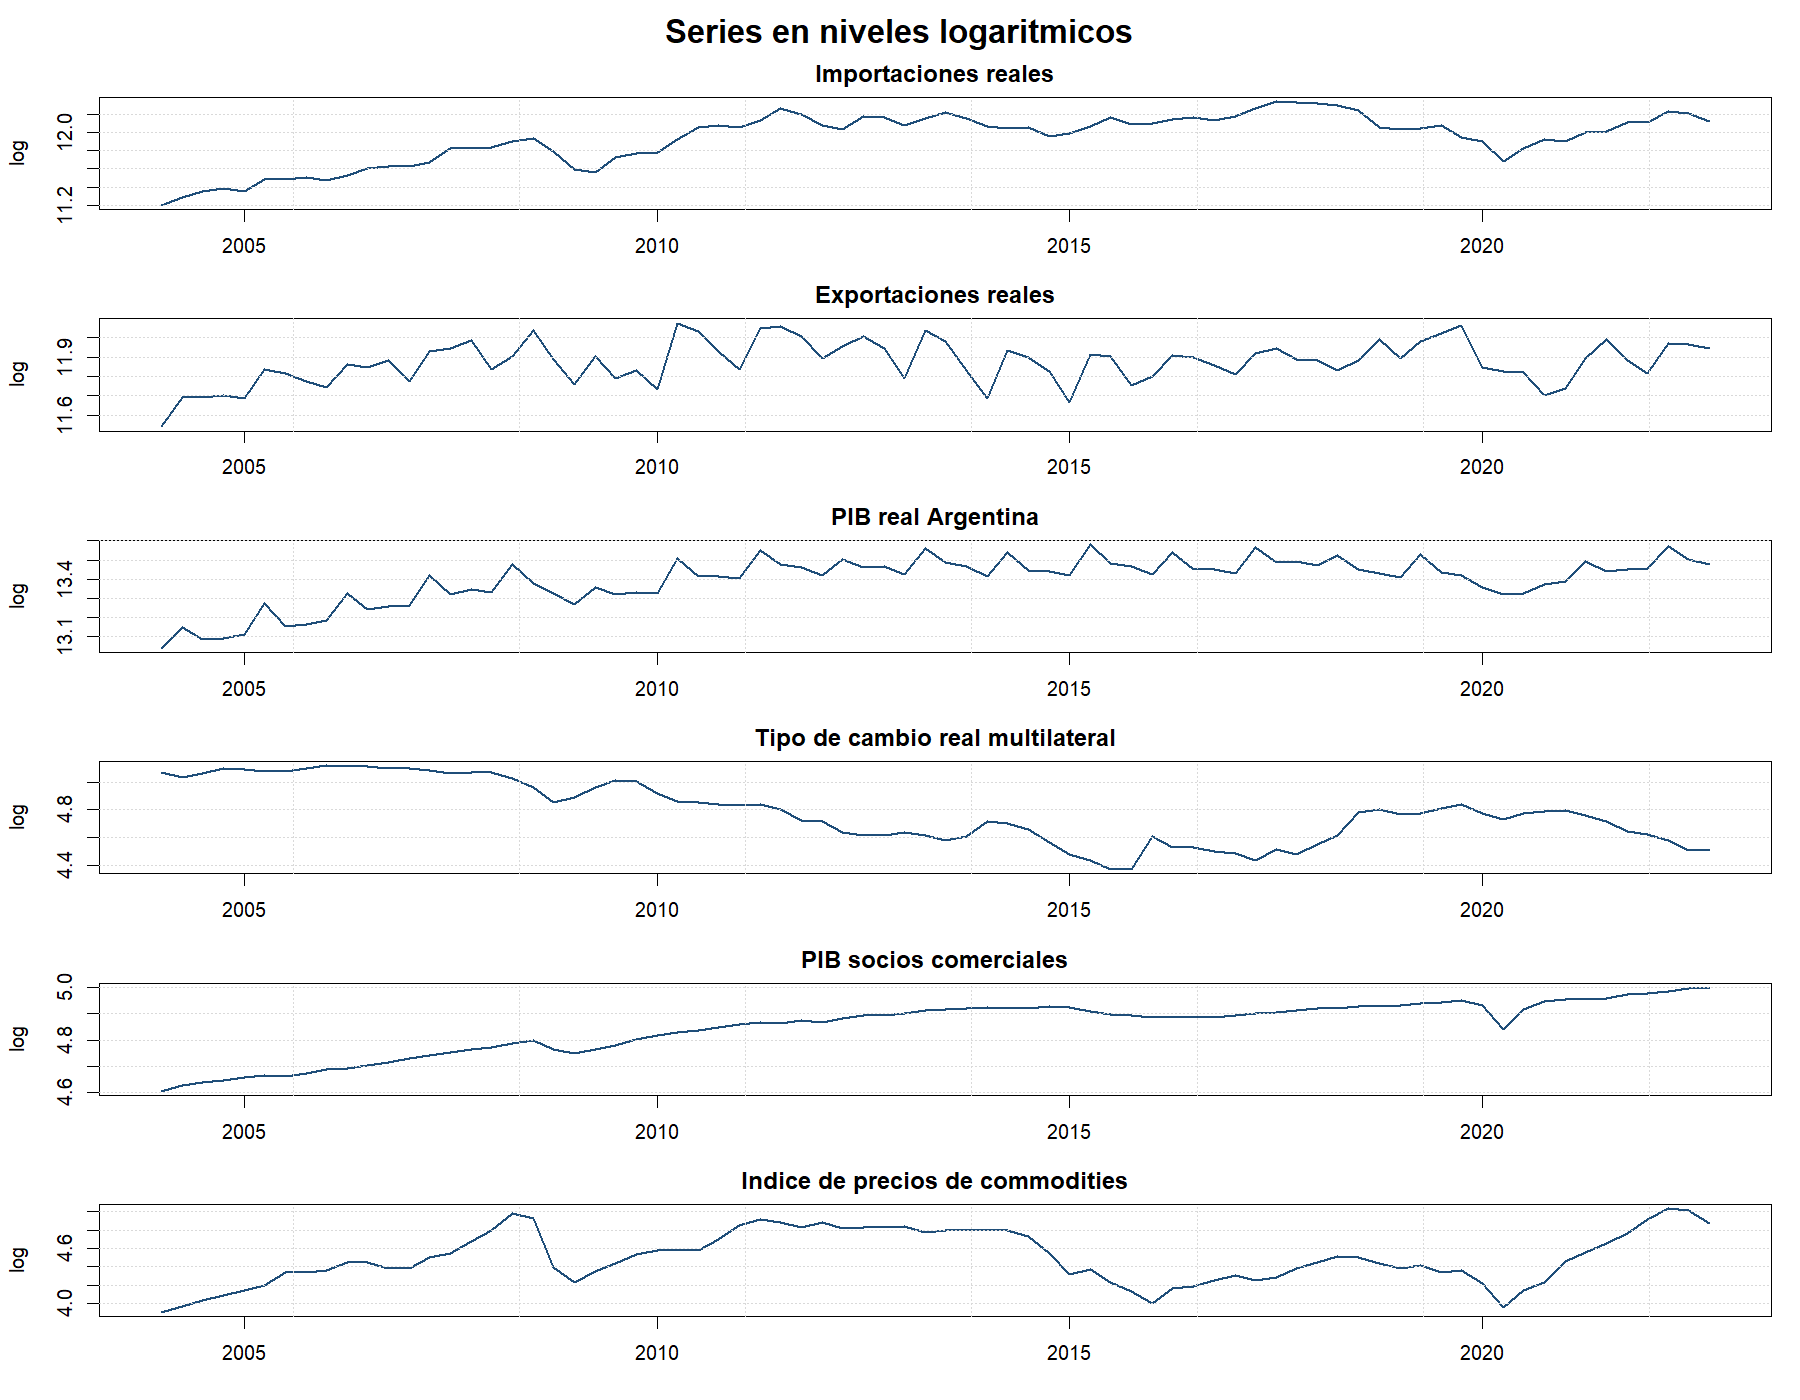
\includegraphics[width=\textwidth]{figure_01_log_levels.png}
\caption{Series en niveles logarítmicos.}
\label{fig:niveles-logaritmicos}
\end{figure}

\autoref{fig:diferencias-logaritmicas} muestra las primeras diferencias
logarítmicas. Esta transformación concentra la atención en la dinámica de corto
plazo y permite observar con más claridad los episodios de mayor volatilidad. En
la muestra base, las exportaciones presentan la mayor desviación estándar
trimestral en diferencias, seguidas por importaciones y PIB argentino. El PIB de
socios comerciales es la serie menos volátil, como era esperable por tratarse de
un indicador externo agregado.

\begin{figure}[H]
\centering
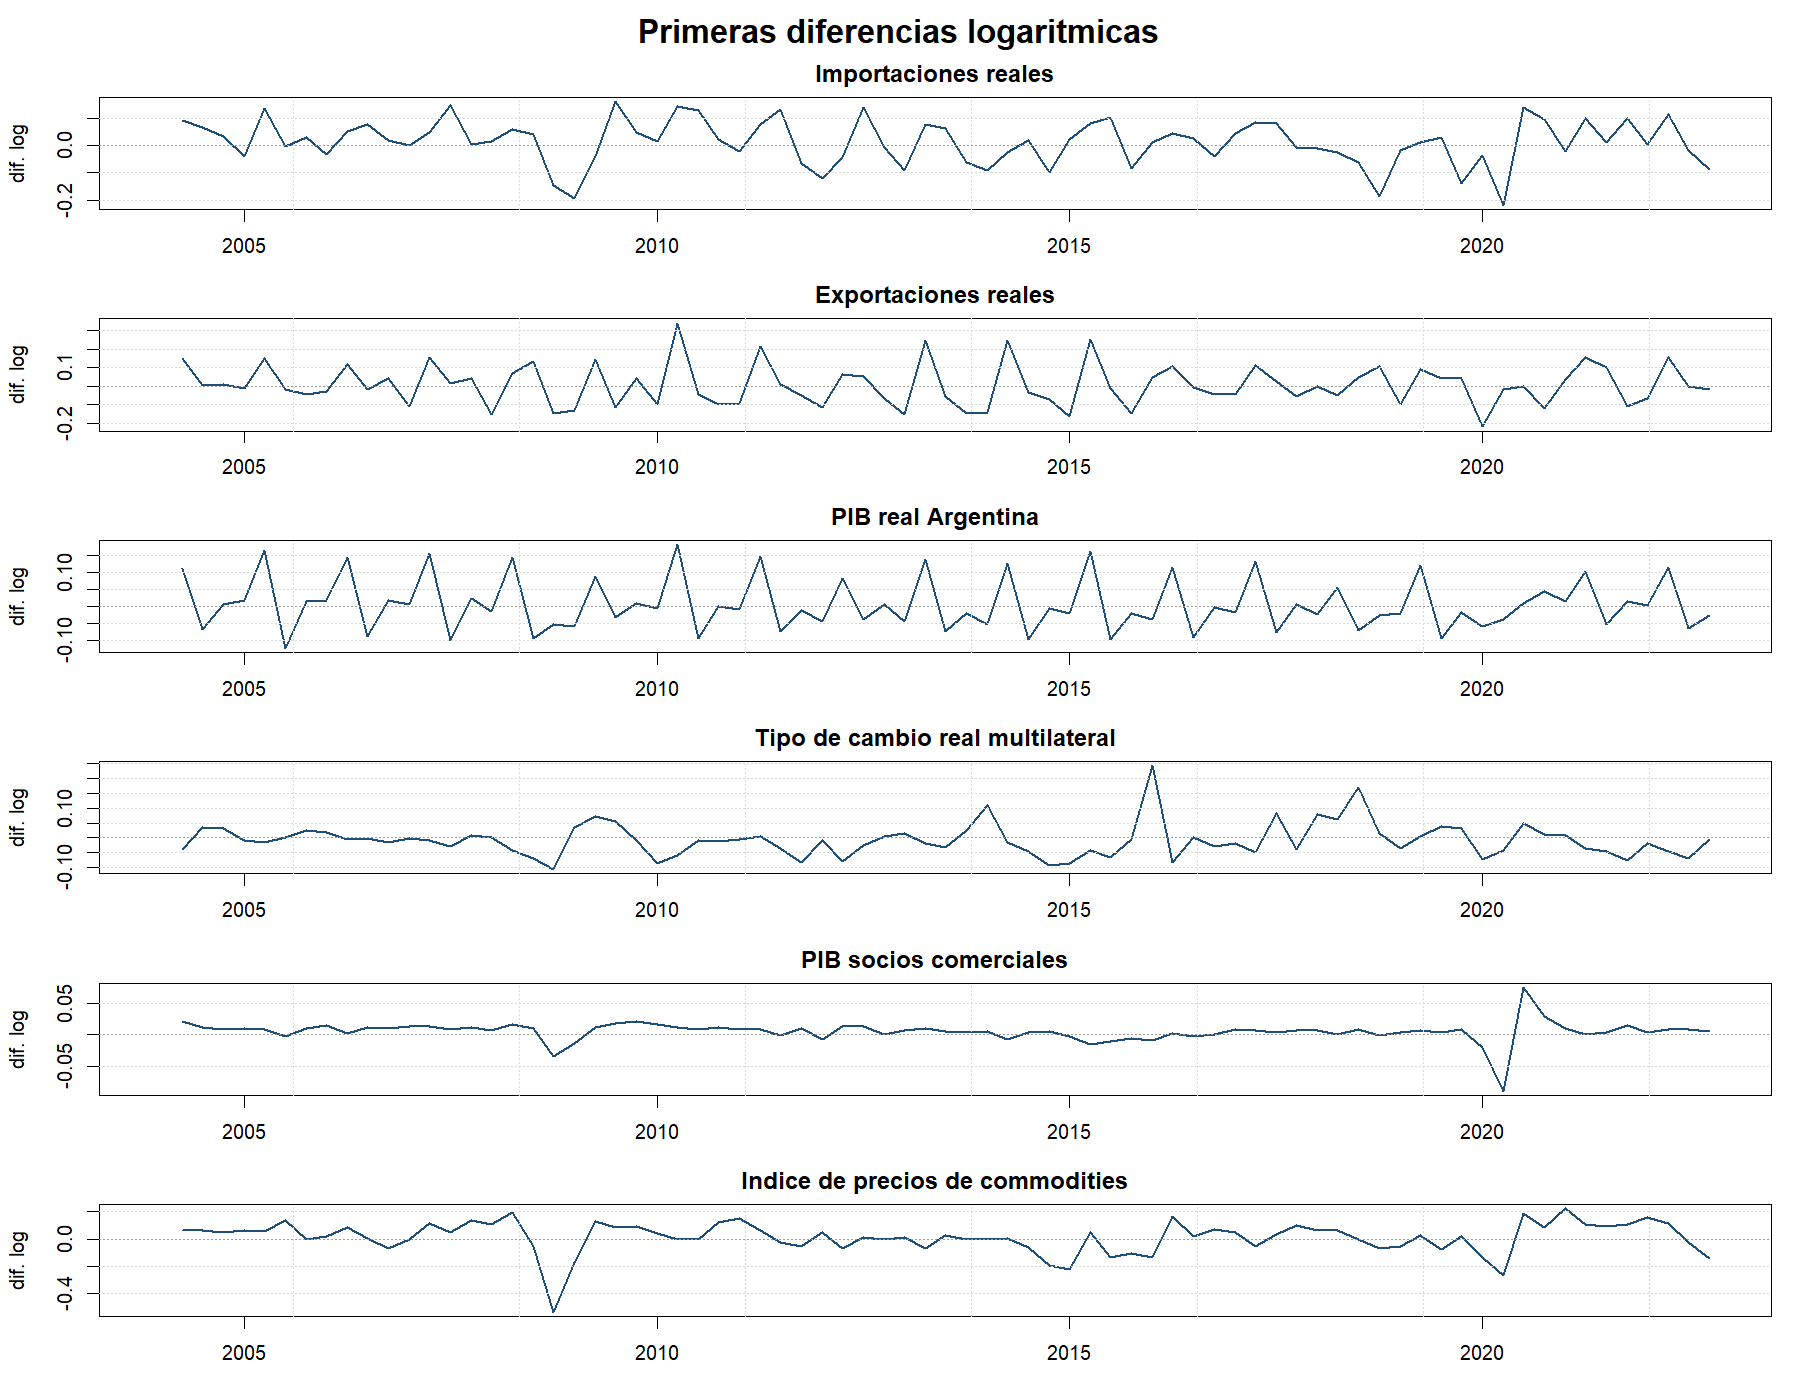
\includegraphics[width=\textwidth]{figure_02_log_differences.png}
\caption{Primeras diferencias logarítmicas.}
\label{fig:diferencias-logaritmicas}
\end{figure}

\autoref{tab:resumen-descriptivo} sintetiza la amplitud de las series en niveles
logarítmicos y la media y volatilidad de las primeras diferencias. Estos
indicadores resumen numéricamente los patrones observados en las figuras
anteriores.

\begin{table}[H]
\centering
\caption{Resumen descriptivo de variables principales.}
\label{tab:resumen-descriptivo}
\small
\begin{tabular}{lrrr}
\toprule
Serie & Rango en nivel log. & Media dif. log. & Desv. est. dif. log. \\
\midrule
Importaciones reales & 1.1426 & 0.0123 & 0.0838 \\
Exportaciones reales & 0.5356 & 0.0054 & 0.1140 \\
PIB real Argentina & 0.5416 & 0.0058 & 0.0784 \\
ITCRM & 0.7483 & -0.0075 & 0.0566 \\
PIB socios comerciales & 0.3964 & 0.0053 & 0.0168 \\
\bottomrule
\end{tabular}
\end{table}

El análisis por trimestre de las diferencias logarítmicas se conserva en el
anexo de salidas para revisar patrones estacionales. En esta etapa descriptiva,
los gráficos sugieren que la modelización debe permitir tanto persistencia en
niveles como shocks transitorios relevantes, lo que justifica continuar con las
pruebas de raíz unitaria, cointegración y modelos dinámicos.

\subsection{Pruebas de integración}
\label{subsec:resultados-integracion}

\noindent\textit{Nota metodológica.} Las pruebas ADF se estiman con
\texttt{urca::ur.df} y deben contrastarse con la rutina de clase
\texttt{Test.ADF.Ver.3.R} antes de cerrar la versión final. En niveles
logarítmicos se utiliza una especificación con tendencia determinística; en
primeras diferencias logarítmicas se utiliza una especificación con constante.
En ambos casos se emplean cuatro rezagos fijos. La clasificación final del orden
de integración deberá revisar también la sensibilidad al criterio de selección
de rezagos de la función del curso.

\autoref{tab:adf-resultados-formales} presenta los estadísticos ADF para cada
serie en niveles logarítmicos y primeras diferencias.

\begin{table}[H]
\centering
\caption{Pruebas ADF formales en niveles y primeras diferencias.}
\label{tab:adf-resultados-formales}
\small
\resizebox{\textwidth}{!}{%
\begin{tabular}{l l c c r r r l}
\toprule
Serie & Transformación & Det. & Obs. & Rezagos & Estadístico & VC 5\% & Decisión 5\% \\
\midrule
Importaciones reales & Nivel log. & Tend. & 76 & 4 & -2.841 & -3.450 & No rechaza raíz unitaria \\
Importaciones reales & Dif. log. & Const. & 75 & 4 & -3.847 & -2.890 & Rechaza raíz unitaria \\
Exportaciones reales & Nivel log. & Tend. & 76 & 4 & -3.530 & -3.450 & Rechaza raíz unitaria \\
Exportaciones reales & Dif. log. & Const. & 75 & 4 & -4.267 & -2.890 & Rechaza raíz unitaria \\
PIB real Argentina & Nivel log. & Tend. & 76 & 4 & -2.923 & -3.450 & No rechaza raíz unitaria \\
PIB real Argentina & Dif. log. & Const. & 75 & 4 & -4.036 & -2.890 & Rechaza raíz unitaria \\
ITCRM & Nivel log. & Tend. & 76 & 4 & -1.662 & -3.450 & No rechaza raíz unitaria \\
ITCRM & Dif. log. & Const. & 75 & 4 & -4.125 & -2.890 & Rechaza raíz unitaria \\
PIB socios comerciales & Nivel log. & Tend. & 76 & 4 & -1.982 & -3.450 & No rechaza raíz unitaria \\
PIB socios comerciales & Dif. log. & Const. & 75 & 4 & -3.875 & -2.890 & Rechaza raíz unitaria \\
\bottomrule
\end{tabular}%
}
\end{table}

\autoref{tab:orden-integracion-formal} traduce los resultados ADF en una
clasificación operativa del orden de integración de cada serie.

\begin{table}[H]
\centering
\caption{Orden de integración formal según ADF.}
\label{tab:orden-integracion-formal}
\small
\begin{tabular}{lccc}
\toprule
Serie & Nivel logarítmico & Primera diferencia & Orden formal \\
\midrule
Importaciones reales & No rechaza raíz unitaria & Rechaza raíz unitaria & I(1) \\
Exportaciones reales & Rechaza raíz unitaria & Rechaza raíz unitaria & I(0) \\
PIB real Argentina & No rechaza raíz unitaria & Rechaza raíz unitaria & I(1) \\
ITCRM & No rechaza raíz unitaria & Rechaza raíz unitaria & I(1) \\
PIB socios comerciales & No rechaza raíz unitaria & Rechaza raíz unitaria & I(1) \\
\bottomrule
\end{tabular}
\end{table}

\subsection{Resultados Engle-Granger y ECM}
\label{subsec:resultados-eg-ecm}

\noindent\textit{Nota metodológica.} En esta etapa se reestima la línea
uniecuacional del TP 2 con la muestra base del TP 3. Primero se estiman las
ecuaciones de largo plazo por MCO y luego se aplica una prueba ADF sobre los
residuos, sin constante, comparando el estadístico con los valores críticos de
Engle-Granger utilizados en clase. La consigna permite una lectura flexible al
10\% para la evidencia de cointegración. Cuando los residuos son estacionarios
se estima un ECM; cuando no lo son, se conserva un modelo en primeras
diferencias y las elasticidades de largo plazo se reportan solo como
indicativas. En la versión final debe agregarse la verificación del vector de
cointegración según Wickens y Breusch para el enfoque Engle-Granger.

\autoref{tab:engle-granger-residuos} reporta la prueba sobre los residuos de
las ecuaciones de largo plazo y permite decidir si corresponde estimar un ECM.

\begin{table}[H]
\centering
\caption{Pruebas Engle-Granger sobre residuos.}
\label{tab:engle-granger-residuos}
\small
\begin{tabular}{lrrrrl}
\toprule
Sistema & Obs. & Rezagos ADF & Estadístico & VC 5\% & Decisión 5\% \\
\midrule
Importaciones & 76 & 4 & -4.558 & -3.930 & Cointegración \\
Exportaciones & 76 & 4 & -3.308 & -3.930 & Sin cointegración \\
\bottomrule
\end{tabular}
\end{table}

\autoref{tab:elasticidades-eg-ecm} sintetiza las elasticidades de largo plazo
de Engle-Granger y las elasticidades de corto plazo de los modelos ECM o en
diferencias.

\begin{table}[H]
\centering
\caption{Elasticidades estimadas por Engle-Granger y ECM.}
\label{tab:elasticidades-eg-ecm}
\small
\resizebox{\textwidth}{!}{%
\begin{tabular}{lcccp{5.8cm}}
\toprule
Flujo & Variable & Largo plazo & Corto plazo & Interpretación \\
\midrule
Importaciones & PIB & 1.518 & 0.493 & Elasticidad ingreso positiva; ECM estimado por evidencia de cointegración. \\
Importaciones & TCR & -0.399 & -0.057 & Elasticidad cambiaria negativa; ECM estimado por evidencia de cointegración. \\
Exportaciones & PIB socios & 0.720 & -0.305 & Largo plazo solo indicativo; el modelo operativo queda en diferencias. \\
Exportaciones & TCR & 0.159 & -0.113 & Largo plazo solo indicativo; el modelo operativo queda en diferencias. \\
\bottomrule
\end{tabular}
}
\end{table}

En importaciones, el estadístico ADF sobre los residuos de la ecuación de largo
plazo es menor que el valor crítico de Engle-Granger al 5\%, por lo que se
mantiene la evidencia de cointegración y se estima un ECM. El coeficiente del
término de corrección del error rezagado es \(-0.525\), con valor p menor a
0.001, lo que implica una velocidad de ajuste trimestral aproximada de 52.5\%.

En exportaciones, los residuos de la ecuación de largo plazo no rechazan la
hipótesis de raíz unitaria con los valores críticos de Engle-Granger. Por ello,
las elasticidades de largo plazo se reportan solo como referencia indicativa y
la especificación operativa se mantiene en primeras diferencias. En ese modelo
base, el índice de commodities se incluye como control de corto plazo, aunque la
cuadro principal conserva las elasticidades asociadas a demanda externa e ITCRM
para facilitar la comparación con las ecuaciones del marco teórico.

La lectura de esta sección deberá actualizarse con una columna explícita al
10\% cuando se incorporen los valores críticos finales utilizados en clase. Ese
criterio no debe reemplazar la evaluación económica y diagnóstica, sino servir
como umbral adicional para clasificar resultados fronterizos.

\subsection{Resultados Johansen y VECM}
\label{subsec:resultados-johansen-vec}

\noindent\textit{Nota metodológica.} Las pruebas de Johansen se estiman con
\texttt{urca::ca.jo}, \texttt{spec = "transitory"} y \texttt{season = 4}. Como
ejercicio de robustez se comparan dos especificaciones determinísticas usadas
en clase: \texttt{ecdet = "const"} y \texttt{ecdet = "none"}. Se reportan la
prueba de traza y la prueba de máximo autovalor al 5\%, con revisión posterior
al 10\% siguiendo la consigna. El rango se lee de forma secuencial desde la
hipótesis \(r=0\). La metodología de Johansen requiere además revisar la
normalidad de los residuos del sistema; si esa condición no se verifica, los
resultados se reportan como evidencia indicativa. En el sistema de
exportaciones, la lectura debe tomarse como indicativa porque la prueba ADF
formal clasificó \texttt{ln\_exports\_real} como I(0).

\autoref{tab:johansen} presenta la prueba de Johansen bajo la especificación
con constante en la relación de cointegración.

\begin{table}[H]
\centering
\caption{Pruebas de cointegración de Johansen: especificación con constante.}
\label{tab:johansen}
\small
\resizebox{\textwidth}{!}{%
\begin{tabular}{lcccccc}
\toprule
Sistema & Rezago VAR & \(K\) Johansen & Traza \(r=0\) & Max. autovalor \(r=0\) & Rango traza & Rango max. \\
\midrule
Importaciones & 4 & 4 & 35.449* & 18.937 & 1 & 0 \\
Exportaciones & 1 & 2 & 39.068* & 19.263 & 1 & 0 \\
\bottomrule
\end{tabular}
}
\caption*{\footnotesize Nota: el asterisco indica rechazo al 5\% de la hipótesis
nula \(r=0\). Los valores críticos al 5\% son 34.91 para la prueba de traza y
22.00 para la prueba de máximo autovalor bajo la especificación utilizada.}
\end{table}

\autoref{tab:johansen-robustez} compara la decisión de rango bajo las
especificaciones determinísticas \texttt{const} y \texttt{none}.

\begin{table}[H]
\centering
\caption{Robustez del rango de Johansen.}
\label{tab:johansen-robustez}
\small
\begin{tabular}{llcccc}
\toprule
Sistema & Especificación & Rezago VAR & \(K\) Johansen & Rango traza & Rango max. \\
\midrule
Importaciones & \texttt{const} & 4 & 4 & 1 & 0 \\
Importaciones & \texttt{none} & 4 & 4 & 1 & 0 \\
Exportaciones & \texttt{const} & 1 & 2 & 1 & 0 \\
Exportaciones & \texttt{none} & 1 & 2 & 0 & 0 \\
\bottomrule
\end{tabular}
\end{table}

\autoref{tab:decision-var-vec} combina la evidencia de integración,
Engle-Granger y Johansen para fijar el tratamiento operativo de cada sistema.

\begin{table}[H]
\centering
\caption{Decisión operativa para VAR/VEC.}
\label{tab:decision-var-vec}
\small
\resizebox{\textwidth}{!}{%
\begin{tabular}{lcccp{6.6cm}}
\toprule
Sistema & ADF dep. & Engle-Granger & Johansen robusto & Tratamiento recomendado \\
\midrule
Importaciones & I(1) & Sí & Parcial: traza \(r=1\), máximo \(r=0\) &
Estimar VECM con \(r=1\) como extensión multivariada y mantener el ECM como respaldo uniecuacional. \\
Exportaciones & I(0) & No & Débil: solo traza con \texttt{const} sugiere \(r=1\) &
Estimar VAR en diferencias; reportar Johansen solo como evidencia indicativa. \\
\bottomrule
\end{tabular}
}
\end{table}

La comparación de especificaciones permite fijar una regla metodológica para no
sobreinterpretar la evidencia multivariada. En importaciones, la evidencia es
razonablemente favorable a trabajar con una relación de equilibrio: la variable
dependiente es compatible con I(1), Engle-Granger respalda cointegración y la
prueba de traza de Johansen sugiere \(r=1\) tanto con constante como sin
constante. Sin embargo, la prueba de máximo autovalor no confirma ese rango, por
lo que el VECM se usará como extensión multivariada y se contrastará con el ECM
uniecuacional.

En exportaciones, la evidencia no es suficiente para adoptar un VECM como
especificación principal. La variable dependiente fue clasificada como I(0) en
la prueba ADF formal, Engle-Granger no respalda cointegración y el rango \(r=1\)
por Johansen aparece únicamente en la prueba de traza con constante. Bajo la
especificación \texttt{none}, tanto traza como máximo autovalor sugieren rango
cero. Por prudencia, el tratamiento principal para exportaciones será un VAR en
diferencias. No obstante, siguiendo la consigna actualizada, el VECM de
exportaciones deberá reportarse igualmente como ejercicio indicativo, junto con
la advertencia sobre integración y diagnósticos.

\pendiente{Reportar vectores de cointegración normalizados, coeficientes de
ajuste, pruebas de normalidad y elasticidades de corto plazo del VECM. Incluir
importaciones como evidencia principal si los diagnósticos lo permiten y
exportaciones como ejercicio indicativo.}

\subsection{VAR en diferencias e interpretación de corto plazo}
\label{subsec:resultados-var}

\pendiente{Reportar el VAR en diferencias para los sistemas sin cointegración
robusta, especialmente exportaciones, incluyendo autocorrelación con
\texttt{vcorr\_res.R}, heterocedasticidad, normalidad, estabilidad y exclusión
de rezagos.}

% -------------------------------
% 7. Comparación
% -------------------------------
\section{Comparación de resultados}
\label{sec:comparacion}

La comparación debe distinguir tres niveles. Primero, la comparación interna
entre Engle-Granger y Johansen. Segundo, la comparación entre elasticidades de
largo y corto plazo. Tercero, la comparación con la literatura aplicada para
Argentina. La consigna enfatiza que esta sección no debe limitarse a contrastar
coeficientes: debe explicar qué resultados son válidos, cuáles son indicativos
y qué implicancias económicas surgen para la restricción externa.

\autoref{tab:comparacion-literatura} organiza la comparación entre los
resultados propios y las referencias aplicadas exigidas por la consigna.

\begin{table}[H]
\centering
\caption{Comparación sintética de elasticidades y literatura.}
\label{tab:comparacion-literatura}
\small
\begin{tabular}{p{3.2cm}p{3.2cm}p{3.2cm}p{4.2cm}}
\toprule
Referencia / método & Importaciones & Exportaciones & Comentario \\
\midrule
Engle-Granger / ECM & PIB: 1.518; TCR: -0.399; ajuste ECM: -0.525 & PIB socios: 0.720; TCR: 0.159 & Importaciones con cointegración; exportaciones solo indicativo en largo plazo. \\
Johansen / VECM & \pendiente{normalizar vector y coeficientes de ajuste} & \pendiente{reportar ejercicio indicativo} & Debe distinguir evidencia principal de ejercicios indicativos. \\
Berrettoni y Castresana (2008) & \pendiente{} & \pendiente{} & \pendiente{} \\
Bus y Nicolini-Llosa (2007) & \pendiente{} & No aplica & \pendiente{} \\
Zack y Sotelsek (2016) & \pendiente{} & \pendiente{} & \pendiente{} \\
Song, Witt y Li (2008) & No aplica directo & No aplica directo & Referencia metodológica para demanda y modelos dinámicos. \\
\bottomrule
\end{tabular}
\end{table}

La primera lectura de los resultados mantiene una asimetría relevante para la
interpretación económica. En importaciones, la elasticidad ingreso de largo
plazo estimada por Engle-Granger es mayor que uno y el ECM muestra un ajuste
significativo hacia el equilibrio. Ese resultado es consistente con la hipótesis
de que el crecimiento interno aumenta con intensidad la demanda de importaciones
y, por lo tanto, puede presionar la restricción externa. En exportaciones, la
evidencia de largo plazo es más débil; por esa razón, la comparación con la
literatura deberá apoyarse principalmente en la magnitud y el signo de los
coeficientes, aclarando que la evidencia econométrica no permite tratarlos como
elasticidades de equilibrio robustas.

\pendiente{Completar los valores de literatura y construir un cuadro final más
expeditivo con elasticidades ingreso, elasticidades cambiarias, metodología,
período muestral y lectura económica.}

% -------------------------------
% 8. Conclusiones
% -------------------------------
\section{Conclusiones}
\label{sec:conclusiones}

Los resultados preliminares indican que la evidencia más sólida aparece en la
ecuación de importaciones. En ese caso, las pruebas uniecuacionales respaldan
cointegración y permiten interpretar la elasticidad ingreso de largo plazo como
un parámetro de equilibrio, complementado por un ECM con velocidad de ajuste
significativa. La evidencia multivariada de Johansen también sugiere una
relación de cointegración por la prueba de traza, aunque el máximo autovalor no
confirma el mismo rango; por lo tanto, el VECM debe utilizarse como extensión y
contraste, no como sustituto automático del resultado Engle-Granger.

Para exportaciones, la evidencia disponible exige mayor cautela. La prueba ADF
formal clasifica la variable dependiente como estacionaria en niveles,
Engle-Granger no confirma cointegración y Johansen solo entrega una señal débil
bajo una especificación determinística. En consecuencia, el modelo principal
debe orientarse hacia elasticidades de corto plazo mediante VAR en diferencias,
mientras que los ejercicios de cointegración y VECM se reportarán con carácter
indicativo. La conclusión económica deberá cerrarse luego de incorporar los
diagnósticos pendientes, la comparación con literatura y las pruebas solicitadas
en la consigna actualizada.

% -------------------------------
% Bibliografía
% -------------------------------
\begin{thebibliography}{99}

\bibitem{berrettoni_castresana_2008}
Berrettoni, D. y Castresana, S. (2008).
\textit{Elasticidades de comercio de la Argentina para el período 1993--2008}.
Revista del CEI: Comercio Exterior e Integración, Nro. 16, 85--97.

\bibitem{bus_nicolini_llosa_2007}
Bus, A. G. y Nicolini-Llosa, J. L. (2007).
\textit{Importaciones de Argentina, una estimación econométrica}.
XLII Reunión Anual de la Asociación Argentina de Economía Política.

\bibitem{enders_2014}
Enders, W. (2014).
\textit{Applied Econometric Time Series}.
4ta ed. Wiley.

\bibitem{engle_granger_1987}
Engle, R. F. y Granger, C. W. J. (1987).
\textit{Co-integration and error correction: representation, estimation, and
testing}.
Econometrica, 55(2), 251--276.

\bibitem{fabris_2026}
Fabris, J. (2026).
\textit{Modelos Econométricos Aplicados: Series de Tiempo}.
Notas de clase, Universidad de Buenos Aires, Facultad de Ciencias Económicas.

\bibitem{hamilton_1994}
Hamilton, J. D. (1994).
\textit{Time Series Analysis}.
Princeton University Press.

\bibitem{johansen_1995}
Johansen, S. (1995).
\textit{Likelihood-Based Inference in Cointegrated Vector Autoregressive Models}.
Oxford University Press.

\bibitem{lutkepohl_2005}
Lütkepohl, H. (2005).
\textit{New Introduction to Multiple Time Series Analysis}.
Springer.

\bibitem{pfaff_2008}
Pfaff, B. (2008).
\textit{Analysis of Integrated and Cointegrated Time Series with R}.
2da ed. Springer.

\bibitem{song_witt_li_2008}
Song, H., Witt, S. F. y Li, G. (2008).
\textit{The advanced econometrics of tourism demand}.
Routledge.

\bibitem{zack_sotelsek_2016}
Zack, G. y Sotelsek, D. (2016).
\textit{Las posibilidades de crecimiento de la Argentina a partir de una
estimación de sus elasticidades de comercio exterior}.
Revista de Economía Política de Buenos Aires, Universidad de Buenos Aires,
Facultad de Ciencias Económicas.

\end{thebibliography}

% -------------------------------
% Anexos
% -------------------------------
\appendix
\section{Anexos}
\label{sec:anexos}

\subsection{Salidas econométricas}
\label{subsec:salidas-econometricas}

\autoref{tab:verificacion-variables} documenta que las variables requeridas
están disponibles en el panel y en la muestra de trabajo.

\begin{table}[H]
\centering
\caption{Verificación de variables en la base de trabajo.}
\label{tab:verificacion-variables}
\small
\begin{tabular}{lcc}
\toprule
Variable & Obs. panel completo & Obs. muestra base \\
\midrule
\texttt{quarter} & 88 & 76 \\
\texttt{year} & 88 & 76 \\
\texttt{q} & 88 & 76 \\
\texttt{quarter\_date} & 88 & 76 \\
\texttt{ln\_imports\_real} & 76 & 76 \\
\texttt{ln\_exports\_real} & 76 & 76 \\
\texttt{ln\_gdp\_real} & 76 & 76 \\
\texttt{ln\_itcrm} & 88 & 76 \\
\texttt{ln\_pib\_socios} & 88 & 76 \\
\texttt{d\_ln\_imports\_real} & 75 & 75 \\
\texttt{d\_ln\_exports\_real} & 75 & 75 \\
\texttt{d\_ln\_gdp\_real} & 75 & 75 \\
\texttt{d\_ln\_itcrm} & 87 & 75 \\
\texttt{d\_ln\_pib\_socios} & 87 & 75 \\
\bottomrule
\end{tabular}
\end{table}

\autoref{tab:outputs-fase-base} enumera los archivos generados por el script y
el contenido de cada salida reproducible.

\begin{table}[H]
\centering
\caption{Archivos generados por la fase base del script.}
\label{tab:outputs-fase-base}
\small
\begin{tabular}{>{\raggedright\arraybackslash}p{6.1cm}>{\raggedright\arraybackslash}p{7.7cm}}
\toprule
Archivo & Contenido \\
\midrule
\path{section_01_model_sample.csv} & Definición de muestra de trabajo \\
\path{section_01_variable_check.csv} & Verificación de variables requeridas \\
\path{section_01_system_samples.csv} & Subconjuntos para sistemas de importaciones y exportaciones \\
\path{section_01_descriptive_statistics.csv} & Estadísticas descriptivas de niveles logarítmicos y primeras diferencias \\
\path{section_01_descriptive_seasonality_by_quarter.csv} & Resumen por trimestre para revisar estacionalidad en diferencias \\
\path{section_01_descriptive_interpretation_guide.csv} & Guía de lectura descriptiva para el informe \\
\path{section_01_unit_root_adf_results.csv} & Resultados ADF en niveles y diferencias \\
\path{section_01_unit_root_adf_order_summary.csv} & Resumen preliminar de orden de integración \\
\path{section_02_unit_root_adf_urca_results.csv} & Resultados ADF formales con \texttt{ur.df} \\
\path{section_02_unit_root_adf_urca_order_summary.csv} & Resumen formal de orden de integración \\
\path{section_03_var_lag_selection.csv} & Rezagos sugeridos por AIC, HQ, SC/BIC y FPE \\
\path{section_03_var_lag_criteria.csv} & Valores de criterios de información para rezagos candidatos \\
\path{section_03_var_lag_decision.csv} & Decisión de rezagos con SC/BIC como criterio principal \\
\path{section_04_johansen_trace_results.csv} & Pruebas de Johansen por estadístico de traza \\
\path{section_04_johansen_eigen_results.csv} & Pruebas de Johansen por máximo autovalor \\
\path{section_04_johansen_rank_decision.csv} & Decisión preliminar de rango de cointegración \\
\path{section_05_engle_granger_equations.csv} & Ecuaciones de largo plazo Engle-Granger \\
\path{section_05_engle_granger_long_run_coefficients.csv} & Coeficientes de largo plazo Engle-Granger \\
\path{section_05_engle_granger_residual_tests.csv} & Pruebas ADF sobre residuos Engle-Granger \\
\path{section_05_engle_granger_decision.csv} & Decisión operativa entre ECM y primeras diferencias \\
\path{section_05_ecm_short_run_model_summary.csv} & Resumen de modelos ECM o primeras diferencias \\
\path{section_05_ecm_short_run_coefficients.csv} & Coeficientes de modelos ECM o primeras diferencias \\
\path{section_05_ecm_adjustment_summary.csv} & Velocidad de ajuste del ECM \\
\path{section_05_eg_ecm_elasticity_summary.csv} & Resumen de elasticidades Engle-Granger y ECM \\
\path{section_06_johansen_robustness_summary.csv} & Robustez de Johansen comparando \texttt{const} y \texttt{none} \\
\path{section_06_var_vec_treatment_decision.csv} & Decisión operativa entre VECM y VAR en diferencias \\
\bottomrule
\end{tabular}
\end{table}

\subsection{Reproducibilidad}
\label{subsec:reproducibilidad}

\autoref{tab:checklist-reproducibilidad-tp3} resume el estado de avance de los
controles de reproducibilidad necesarios para cerrar el TP.

\begin{table}[H]
\centering
\caption{Lista de verificación de reproducibilidad.}
\label{tab:checklist-reproducibilidad-tp3}
\small
\begin{tabular}{p{8.0cm}p{6.0cm}}
\toprule
Control & Estado \\
\midrule
Base del TP 2 reutilizada o actualizada & Ejecutado \\
Variables transformadas a logaritmos & Ejecutado \\
Pruebas ADF ejecutadas & Ejecutado; falta contraste con \texttt{Test.ADF.Ver.3.R} \\
Engle-Granger replicado & Ejecutado \\
Johansen estimado & Ejecutado \\
VECM o VAR en diferencias estimado & Parcial \\
Diagnósticos post-estimación revisados & Parcial; faltan White/Wald o equivalentes \\
Cuadros y figuras exportadas & Parcial \\
Script principal corre sin interrupciones & Ejecutado \\
\bottomrule
\end{tabular}
\end{table}

\autoref{tab:herramientas-clase} registra qué herramientas solicitadas en la
consigna están disponibles y cuáles deben conseguirse o reconstruirse.

\begin{table}[H]
\centering
\caption{Herramientas de clase solicitadas en la consigna actualizada.}
\label{tab:herramientas-clase}
\small
\begin{tabular}{p{5.0cm}p{4.0cm}p{5.5cm}}
\toprule
Herramienta solicitada & Estado en la carpeta de trabajo & Uso previsto \\
\midrule
\texttt{Test.ADF.Ver.3.R} & Disponible como \texttt{Test.ADF\_Ver.3.R} & Contrastar pruebas de raíz unitaria y selección de rezagos ADF. \\
\texttt{vcorr\_res.R} & Disponible & Diagnóstico de autocorrelación en modelos VAR/VEC. \\
\texttt{VAR\_white\_no\_cross.R} & No localizado en materiales locales & Incorporar test de heterocedasticidad o implementación equivalente. \\
\texttt{VAR\_lag\_exclusion\_wald.R} & No localizado en materiales locales & Evaluar exclusión de rezagos mediante restricciones tipo Wald. \\
Paquetes \texttt{svar}, \texttt{urca} y \texttt{lpirfs} & \texttt{urca} usado; \texttt{svar}/\texttt{lpirfs} pendientes según alcance final & Johansen/VEC, ejercicios estructurales o impulso-respuesta si se incorporan. \\
\bottomrule
\end{tabular}
\end{table}

\end{document}
